%
% Szakdolgozatminta az Eszterházy Károly Katolikus Egyetem
% matematika illetve informatika szakos hallgatóinak.
%

\documentclass[
% opciók nélkül: egyoldalas nyomtatás, elektronikus verzió
% twoside,     % kétoldalas nyomtatás
% tocnopagenum,% oldalszámozás a tartalomjegyzék után kezdődik
]{thesis-ekf}
\usepackage[T1]{fontenc}
\PassOptionsToPackage{defaults=hu-min}{magyar.ldf}
\usepackage[magyar]{babel}
\usepackage{mathtools,amssymb,amsthm,pdfpages}
\footnotestyle{rule=fourth}

\newtheorem{tetel}{Tétel}[chapter]
\theoremstyle{definition}
\newtheorem{definicio}[tetel]{Definíció}
\theoremstyle{remark}
\newtheorem{megjegyzes}[tetel]{Megjegyzés}

\begin{document}

\institute{Matematikai és Informatikai Intézet}
\title{Színes szkenner megvalósítása egy egér szenzorral}
\author{Bodnár Máté\\Programtervező informatikus BSc}
\supervisor{Dr. Geda Gábor\\Egyetemi docens}
\city{Eger}
\date{2024}
\maketitle

\tableofcontents

\chapter*{Bevezetés}
\addcontentsline{toc}{chapter}{Bevezetés}


\chapter{Bevezető}

\section{Motiváció}
\section{Célkitűzés}

\chapter{Felhaszánlt technológiák}
\section{Arduino}
\subsection{Arduino család}
Az Arduino egy széleskörűen elterjedt, nyílt forrású fejlesztőplatform. Az Arduinót oktatási céllal hozták létre, de előszeretettel használják otthoni projektekhez, a kisebb automatizálási feladatoktól kezdve az okosotthonok kialakításáig. Ezek mellett ma már az ipari alkalmazások sem ritkák és rengeteg IOT eszköznek is az alapja.
Az Arduino platform része egy elektronikai áramköri lap és a szoftveres környezet. Maga az áramköri lap nagyon sokféle felépítésben megtalálható.


\subsection{Arduino Uno}
\section{Visual Studio}
\section{Github}
\chapter{Hardveres megvalósítás}
\section{ADNS-9800 szenzor}
\subsection{Működése}
\subsection{Adatok beolvasása}
\section{Adatok továbbítása a Visual Studio felé}
\section{Hardveres bekötés}
\chapter{Szoftveres megvalósítás}
\section{3 dimenziós mátrix felhasználása}
\section{Interpoláció}
\subsection{Lineáris interpoláció}
\subsection{Bikubik interpoláció}
\section{Mátrix átalakítása képpé}



\chapter*{Összegzés}
\addcontentsline{toc}{chapter}{Összegzés}

\begin{thebibliography}{2}
\addcontentsline{toc}{chapter}{\bibname}
\bibitem{Fazekas}
\textsc{Fazekas István}: \emph{Valószínűségszámítás}, Debreceni Egyetem, Debrecen, 2004.
\bibitem{Tomacs}
\textsc{Tómács Tibor}: \emph{A valószínűségszámítás alapjai}, Líceum Kiadó, Eger, 2005.
\end{thebibliography}

% Aláírt, szkennelt nyilatkozat beillesztése a szakdolgozat végére
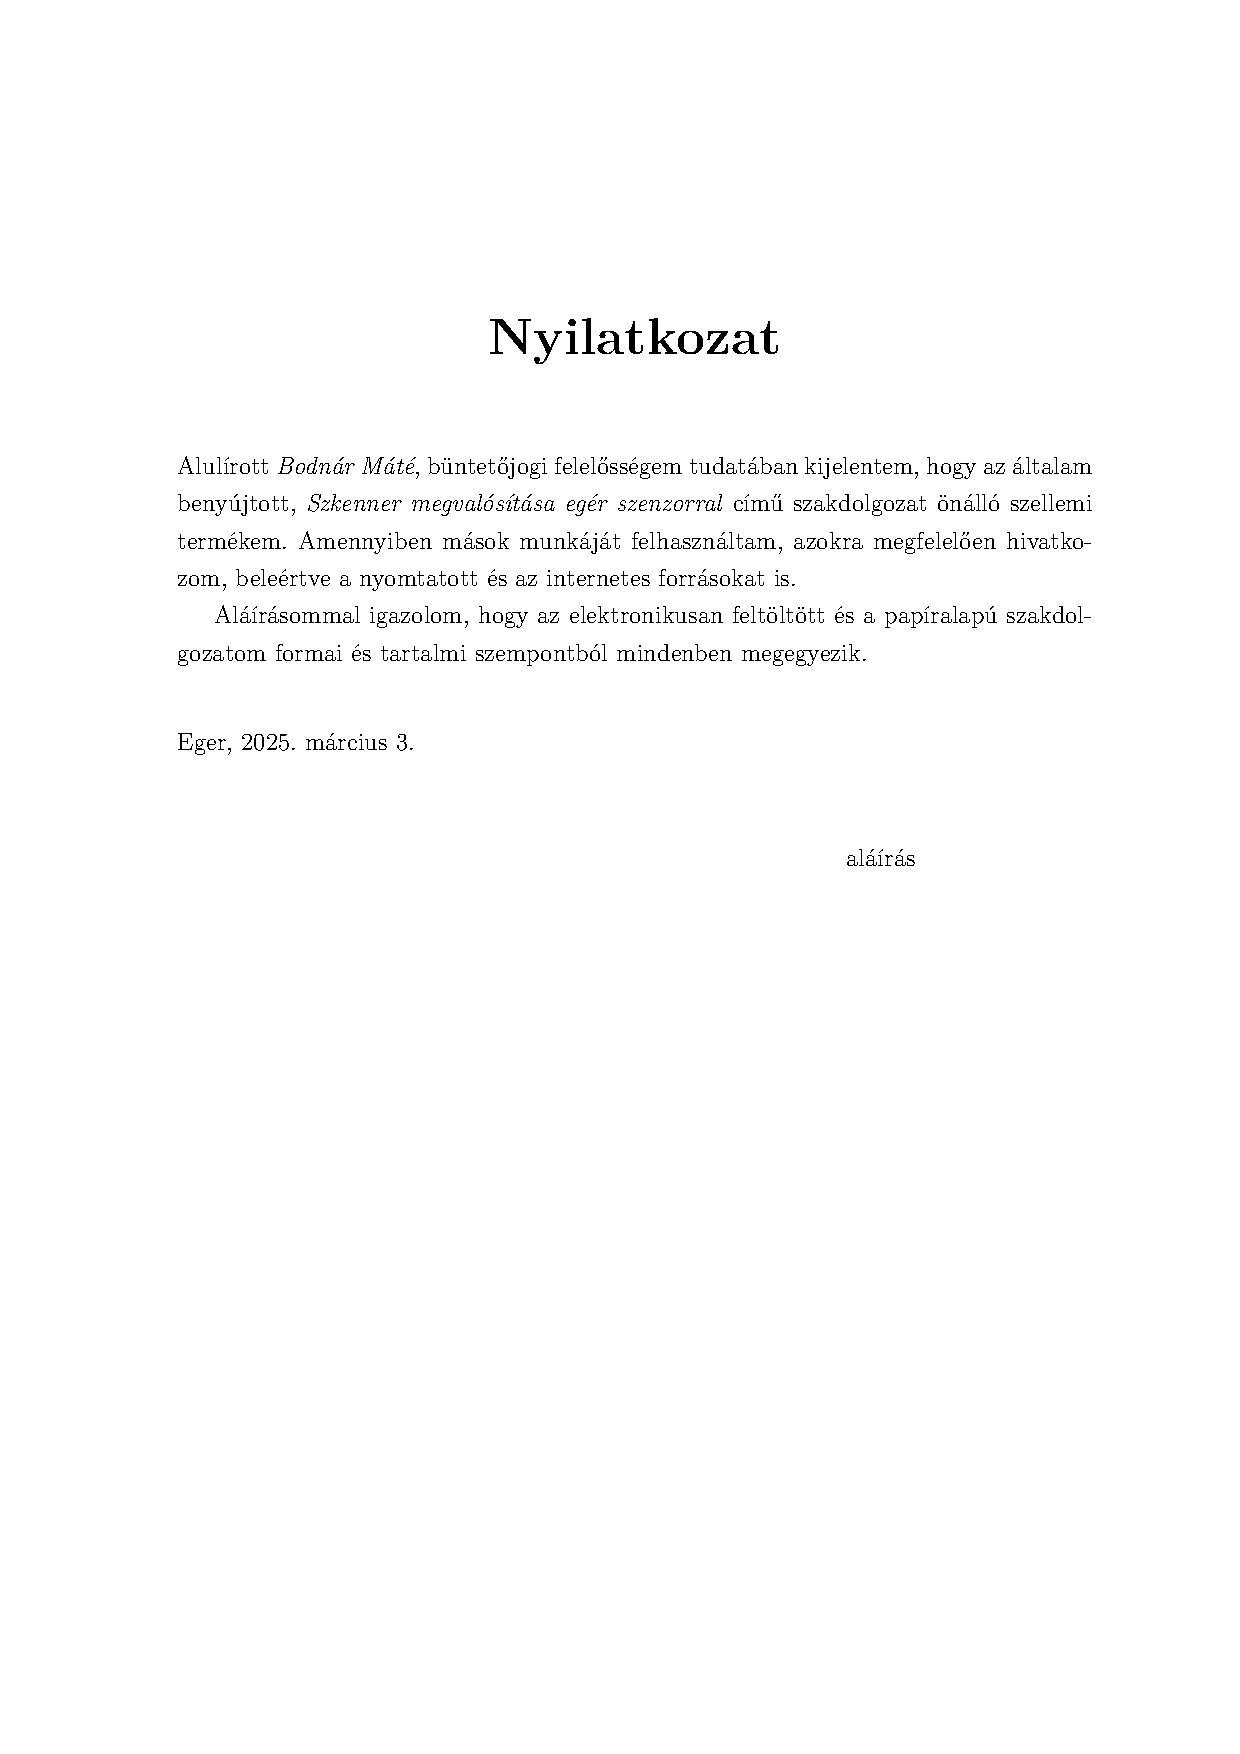
\includepdf{nyilatkozat.pdf}

\end{document}
